\documentclass{standalone}
\usepackage{tikz}
\usetikzlibrary{patterns, positioning}

\begin{document}
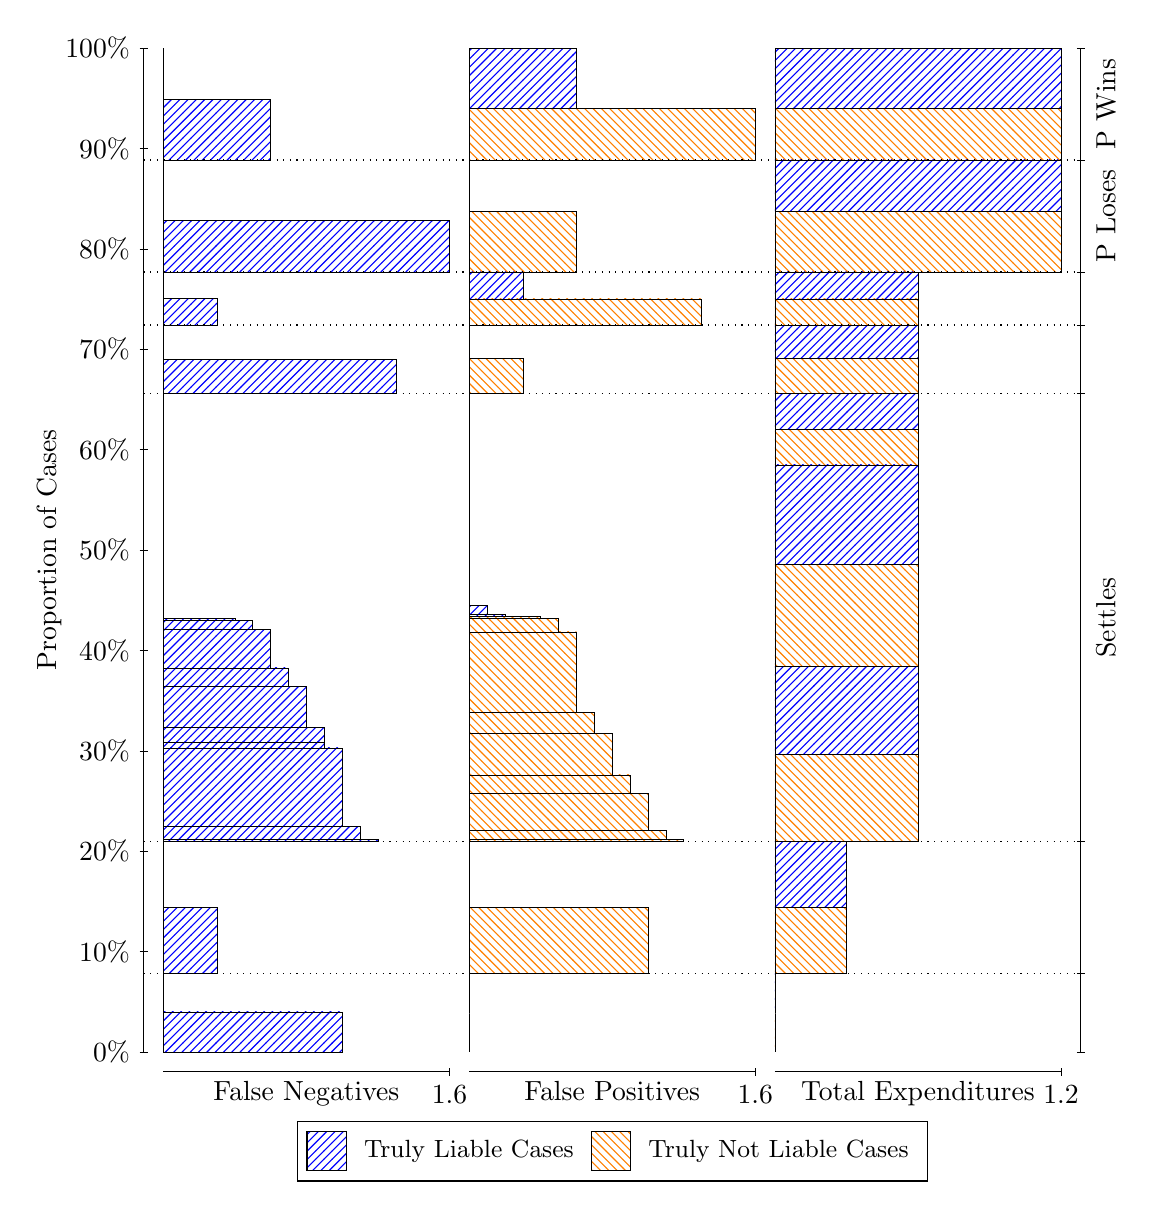
\begin{tikzpicture}
\draw[black, very thin] (1.5,1.75) -- (1.5,14.5);
\node[rotate=90, anchor=center] at (0.3, 8.125) {Proportion of Cases};
\draw[black, very thin] (1.45,1.75) -- (1.55,1.75);
\node[anchor=east] at (1.45, 1.75) {0\%};
\draw[black, very thin] (1.45,3.025) -- (1.55,3.025);
\node[anchor=east] at (1.45, 3.025) {10\%};
\draw[black, very thin] (1.45,4.3) -- (1.55,4.3);
\node[anchor=east] at (1.45, 4.3) {20\%};
\draw[black, very thin] (1.45,5.575) -- (1.55,5.575);
\node[anchor=east] at (1.45, 5.575) {30\%};
\draw[black, very thin] (1.45,6.85) -- (1.55,6.85);
\node[anchor=east] at (1.45, 6.85) {40\%};
\draw[black, very thin] (1.45,8.125) -- (1.55,8.125);
\node[anchor=east] at (1.45, 8.125) {50\%};
\draw[black, very thin] (1.45,9.4) -- (1.55,9.4);
\node[anchor=east] at (1.45, 9.4) {60\%};
\draw[black, very thin] (1.45,10.675) -- (1.55,10.675);
\node[anchor=east] at (1.45, 10.675) {70\%};
\draw[black, very thin] (1.45,11.95) -- (1.55,11.95);
\node[anchor=east] at (1.45, 11.95) {80\%};
\draw[black, very thin] (1.45,13.225) -- (1.55,13.225);
\node[anchor=east] at (1.45, 13.225) {90\%};
\draw[black, very thin] (1.45,14.5) -- (1.55,14.5);
\node[anchor=east] at (1.45, 14.5) {100\%};

\draw[black, very thin] (13.4,1.75) -- (13.4,14.5);
\draw[black, very thin] (13.35,1.75) -- (13.45,1.75);
\node[anchor=west] at (13.35, 1.75) {};
\draw[black, very thin] (13.35,2.7485) -- (13.45,2.7485);
\node[anchor=west] at (13.35, 2.7485) {};
\draw[black, very thin] (13.35,4.4252) -- (13.45,4.4252);
\node[anchor=west] at (13.35, 4.4252) {};
\draw[black, very thin] (13.35,10.113) -- (13.45,10.113);
\node[anchor=west] at (13.35, 10.113) {};
\draw[black, very thin] (13.35,10.982) -- (13.45,10.982);
\node[anchor=west] at (13.35, 10.982) {};
\draw[black, very thin] (13.35,11.656) -- (13.45,11.656);
\node[anchor=west] at (13.35, 11.656) {};
\draw[black, very thin] (13.35,13.078) -- (13.45,13.078);
\node[anchor=west] at (13.35, 13.078) {};
\draw[black, very thin] (13.35,14.5) -- (13.45,14.5);
\node[anchor=west] at (13.35, 14.5) {};

\draw[black, very thin, pattern color=blue, pattern=north east lines] (1.75,1.75) rectangle (4.0208,2.2589);
\draw[black, very thin, pattern color=orange, pattern=north west lines] (1.75,2.2589) rectangle (1.75,2.7485);
\draw[black, very thin, pattern color=blue, pattern=north east lines] (1.75,2.7485) rectangle (2.4312,3.5904);
\draw[black, very thin, pattern color=orange, pattern=north west lines] (1.75,3.5904) rectangle (1.75,4.4252);
\draw[black, very thin, pattern color=blue, pattern=north east lines] (1.75,4.4252) rectangle (4.475,4.4477);
\draw[black, very thin, pattern color=blue, pattern=north east lines] (1.75,4.4477) rectangle (4.2479,4.6133);
\draw[black, very thin, pattern color=blue, pattern=north east lines] (1.75,4.6133) rectangle (4.0208,5.6117);
\draw[black, very thin, pattern color=blue, pattern=north east lines] (1.75,5.6117) rectangle (3.7937,5.6884);
\draw[black, very thin, pattern color=blue, pattern=north east lines] (1.75,5.6884) rectangle (3.7937,5.8762);
\draw[black, very thin, pattern color=blue, pattern=north east lines] (1.75,5.8762) rectangle (3.5667,6.3944);
\draw[black, very thin, pattern color=blue, pattern=north east lines] (1.75,6.3944) rectangle (3.3396,6.6285);
\draw[black, very thin, pattern color=blue, pattern=north east lines] (1.75,6.6285) rectangle (3.1125,7.1137);
\draw[black, very thin, pattern color=blue, pattern=north east lines] (1.75,7.1137) rectangle (2.8854,7.2281);
\draw[black, very thin, pattern color=blue, pattern=north east lines] (1.75,7.2281) rectangle (2.6583,7.2579);
\draw[black, very thin, pattern color=orange, pattern=north west lines] (1.75,7.2579) rectangle (1.75,10.113);
\draw[black, very thin, pattern color=blue, pattern=north east lines] (1.75,10.113) rectangle (4.7021,10.541);
\draw[black, very thin, pattern color=orange, pattern=north west lines] (1.75,10.541) rectangle (1.75,10.982);
\draw[black, very thin, pattern color=blue, pattern=north east lines] (1.75,10.982) rectangle (2.4312,11.325);
\draw[black, very thin, pattern color=orange, pattern=north west lines] (1.75,11.325) rectangle (1.75,11.656);
\draw[black, very thin, pattern color=blue, pattern=north east lines] (1.75,11.656) rectangle (5.3833,12.308);
\draw[black, very thin, pattern color=orange, pattern=north west lines] (1.75,12.308) rectangle (1.75,13.078);
\draw[black, very thin, pattern color=blue, pattern=north east lines] (1.75,13.078) rectangle (3.1125,13.846);
\draw[black, very thin, pattern color=orange, pattern=north west lines] (1.75,13.846) rectangle (1.75,14.5);
\draw[black, very thin, pattern color=orange, pattern=north west lines] (5.6333,1.75) rectangle (5.6333,2.2396);
\draw[black, very thin, pattern color=blue, pattern=north east lines] (5.6333,2.2396) rectangle (5.6333,2.7485);
\draw[black, very thin, pattern color=orange, pattern=north west lines] (5.6333,2.7485) rectangle (7.9042,3.5833);
\draw[black, very thin, pattern color=blue, pattern=north east lines] (5.6333,3.5833) rectangle (5.6333,4.4252);
\draw[black, very thin, pattern color=orange, pattern=north west lines] (5.6333,4.4252) rectangle (8.3583,4.4545);
\draw[black, very thin, pattern color=orange, pattern=north west lines] (5.6333,4.4545) rectangle (8.1313,4.5636);
\draw[black, very thin, pattern color=orange, pattern=north west lines] (5.6333,4.5636) rectangle (7.9042,5.0389);
\draw[black, very thin, pattern color=orange, pattern=north west lines] (5.6333,5.0389) rectangle (7.6771,5.2699);
\draw[black, very thin, pattern color=orange, pattern=north west lines] (5.6333,5.2699) rectangle (7.45,5.7934);
\draw[black, very thin, pattern color=orange, pattern=north west lines] (5.6333,5.7934) rectangle (7.2229,6.0665);
\draw[black, very thin, pattern color=orange, pattern=north west lines] (5.6333,6.0665) rectangle (6.9958,7.0857);
\draw[black, very thin, pattern color=orange, pattern=north west lines] (5.6333,7.0857) rectangle (6.7687,7.2568);
\draw[black, very thin, pattern color=orange, pattern=north west lines] (5.6333,7.2568) rectangle (6.5417,7.2802);
\draw[black, very thin, pattern color=blue, pattern=north east lines] (5.6333,7.2802) rectangle (6.0875,7.31);
\draw[black, very thin, pattern color=blue, pattern=north east lines] (5.6333,7.31) rectangle (5.8604,7.4244);
\draw[black, very thin, pattern color=blue, pattern=north east lines] (5.6333,7.4244) rectangle (5.6333,10.113);
\draw[black, very thin, pattern color=orange, pattern=north west lines] (5.6333,10.113) rectangle (6.3146,10.554);
\draw[black, very thin, pattern color=blue, pattern=north east lines] (5.6333,10.554) rectangle (5.6333,10.982);
\draw[black, very thin, pattern color=orange, pattern=north west lines] (5.6333,10.982) rectangle (8.5854,11.313);
\draw[black, very thin, pattern color=blue, pattern=north east lines] (5.6333,11.313) rectangle (6.3146,11.656);
\draw[black, very thin, pattern color=orange, pattern=north west lines] (5.6333,11.656) rectangle (6.9958,12.426);
\draw[black, very thin, pattern color=blue, pattern=north east lines] (5.6333,12.426) rectangle (5.6333,13.078);
\draw[black, very thin, pattern color=orange, pattern=north west lines] (5.6333,13.078) rectangle (9.2667,13.732);
\draw[black, very thin, pattern color=blue, pattern=north east lines] (5.6333,13.732) rectangle (6.9958,14.5);
\draw[black, very thin, pattern color=orange, pattern=north west lines] (9.5167,1.75) rectangle (9.5167,2.2396);
\draw[black, very thin, pattern color=blue, pattern=north east lines] (9.5167,2.2396) rectangle (9.5167,2.7485);
\draw[black, very thin, pattern color=orange, pattern=north west lines] (9.5167,2.7485) rectangle (10.425,3.5833);
\draw[black, very thin, pattern color=blue, pattern=north east lines] (9.5167,3.5833) rectangle (10.425,4.4252);
\draw[black, very thin, pattern color=orange, pattern=north west lines] (9.5167,4.4252) rectangle (11.333,5.533);
\draw[black, very thin, pattern color=blue, pattern=north east lines] (9.5167,5.533) rectangle (11.333,6.6507);
\draw[black, very thin, pattern color=orange, pattern=north west lines] (9.5167,6.6507) rectangle (11.333,7.943);
\draw[black, very thin, pattern color=blue, pattern=north east lines] (9.5167,7.943) rectangle (11.333,9.2062);
\draw[black, very thin, pattern color=orange, pattern=north west lines] (9.5167,9.2062) rectangle (11.333,9.6612);
\draw[black, very thin, pattern color=blue, pattern=north east lines] (9.5167,9.6612) rectangle (11.333,10.113);
\draw[black, very thin, pattern color=orange, pattern=north west lines] (9.5167,10.113) rectangle (11.333,10.554);
\draw[black, very thin, pattern color=blue, pattern=north east lines] (9.5167,10.554) rectangle (11.333,10.982);
\draw[black, very thin, pattern color=orange, pattern=north west lines] (9.5167,10.982) rectangle (11.333,11.313);
\draw[black, very thin, pattern color=blue, pattern=north east lines] (9.5167,11.313) rectangle (11.333,11.656);
\draw[black, very thin, pattern color=orange, pattern=north west lines] (9.5167,11.656) rectangle (13.15,12.426);
\draw[black, very thin, pattern color=blue, pattern=north east lines] (9.5167,12.426) rectangle (13.15,13.078);
\draw[black, very thin, pattern color=orange, pattern=north west lines] (9.5167,13.078) rectangle (13.15,13.732);
\draw[black, very thin, pattern color=blue, pattern=north east lines] (9.5167,13.732) rectangle (13.15,14.5);
\draw[black, dotted] (1.5,2.7485) -- (13.4,2.7485);
\draw[black, dotted] (1.5,4.4252) -- (13.4,4.4252);
\draw[black, dotted] (1.5,10.113) -- (13.4,10.113);
\draw[black, dotted] (1.5,10.982) -- (13.4,10.982);
\draw[black, dotted] (1.5,11.656) -- (13.4,11.656);
\draw[black, dotted] (1.5,13.078) -- (13.4,13.078);
\draw[black, very thin] (1.75,1.5) -- (5.3833,1.5);
\node[anchor=north] at (3.5667, 1.5) {False Negatives};
\draw[black, very thin] (5.3833,1.45) -- (5.3833,1.55);
\node[anchor=north] at (5.3833, 1.45) {1.6};

\draw[black, very thin] (5.6333,1.5) -- (9.2667,1.5);
\node[anchor=north] at (7.45, 1.5) {False Positives};
\draw[black, very thin] (9.2667,1.45) -- (9.2667,1.55);
\node[anchor=north] at (9.2667, 1.45) {1.6};

\draw[black, very thin] (9.5167,1.5) -- (13.15,1.5);
\node[anchor=north] at (11.333, 1.5) {Total Expenditures};
\draw[black, very thin] (13.15,1.45) -- (13.15,1.55);
\node[anchor=north] at (13.15, 1.45) {1.2};



\node[black, centered, rotate=90] at (13.72, 7.269) {Settles};


\node[black, centered, rotate=90] at (13.72, 12.367) {P Loses};
\node[black, centered, rotate=90] at (13.72, 13.789) {P Wins};

\draw (7.449999999999999,1.5) node[draw=none] (baseCoordinate) {};
\begin{scope}[align=center]
        \matrix[scale=0.5, draw=black, below=0.5cm of baseCoordinate, nodes={draw}, column sep=0.1cm]{
            \node[rectangle, draw, minimum width=0.5cm, minimum height=0.5cm, pattern=north east lines, pattern color=blue] {}; &
            \node[draw=none, font=\small] (B) {Truly Liable Cases}; &
            \node[rectangle, draw, minimum width=0.5cm, minimum height=0.5cm, pattern=north west lines, pattern color=orange] {}; &
            \node[draw=none, font=\small] (B) {Truly Not Liable Cases}; \\
            };
\end{scope}

\end{tikzpicture}
\end{document}